\chapter{Ứng dụng thực tế}
\section{Giới thiệu chung về hệ thống}

\subsection{Mục tiêu thực hiện}

Dự án hướng đến việc xây dựng một hệ thống chatbot tuyển sinh thông minh nhằm hỗ trợ thí sinh và phụ huynh tiếp cận thông tin tuyển sinh một cách chủ động, nhanh chóng và chính xác, mà không cần phải gửi email, gọi điện hoặc nhắn tin qua fanpage của nhà trường để được phản hồi thủ công.

\subsection{Hướng dẫn sử dụng hệ thống}

Hệ thống chatbot được triển khai dưới dạng giao diện web tương tác, cho phép người dùng đặt câu hỏi trực tiếp mà không cần đăng nhập tài khoản. Mỗi phiên làm việc được khởi tạo mới khi tải lại trang, hệ thống có tích hợp lưu trữ lịch sử hội thoại trong phiên hiện tại để hiểu và xử lý ngữ cảnh liên tục.

Sau khi người dùng gửi truy vấn, hệ thống thực hiện các bước:
\begin{itemize}
    \item Truy vấn được mã hóa thành vector ngữ nghĩa và so khớp với các đoạn văn bản trong cơ sở dữ liệu.
    \item Tính điểm và lọc các kết quả không đủ ngưỡng tin cậy.
    \item Truyền các tài liệu vào mô hình ngôn ngữ lớn (LLM) để mô hình tạo ra phản hồi với các tri thức có được từ các tài liệu.
\end{itemize}

\begin{figure}[H]
    \caption{Giao diện hội thoại chatbot truy xuất thông tin tuyển sinh}
    \begin{center}
    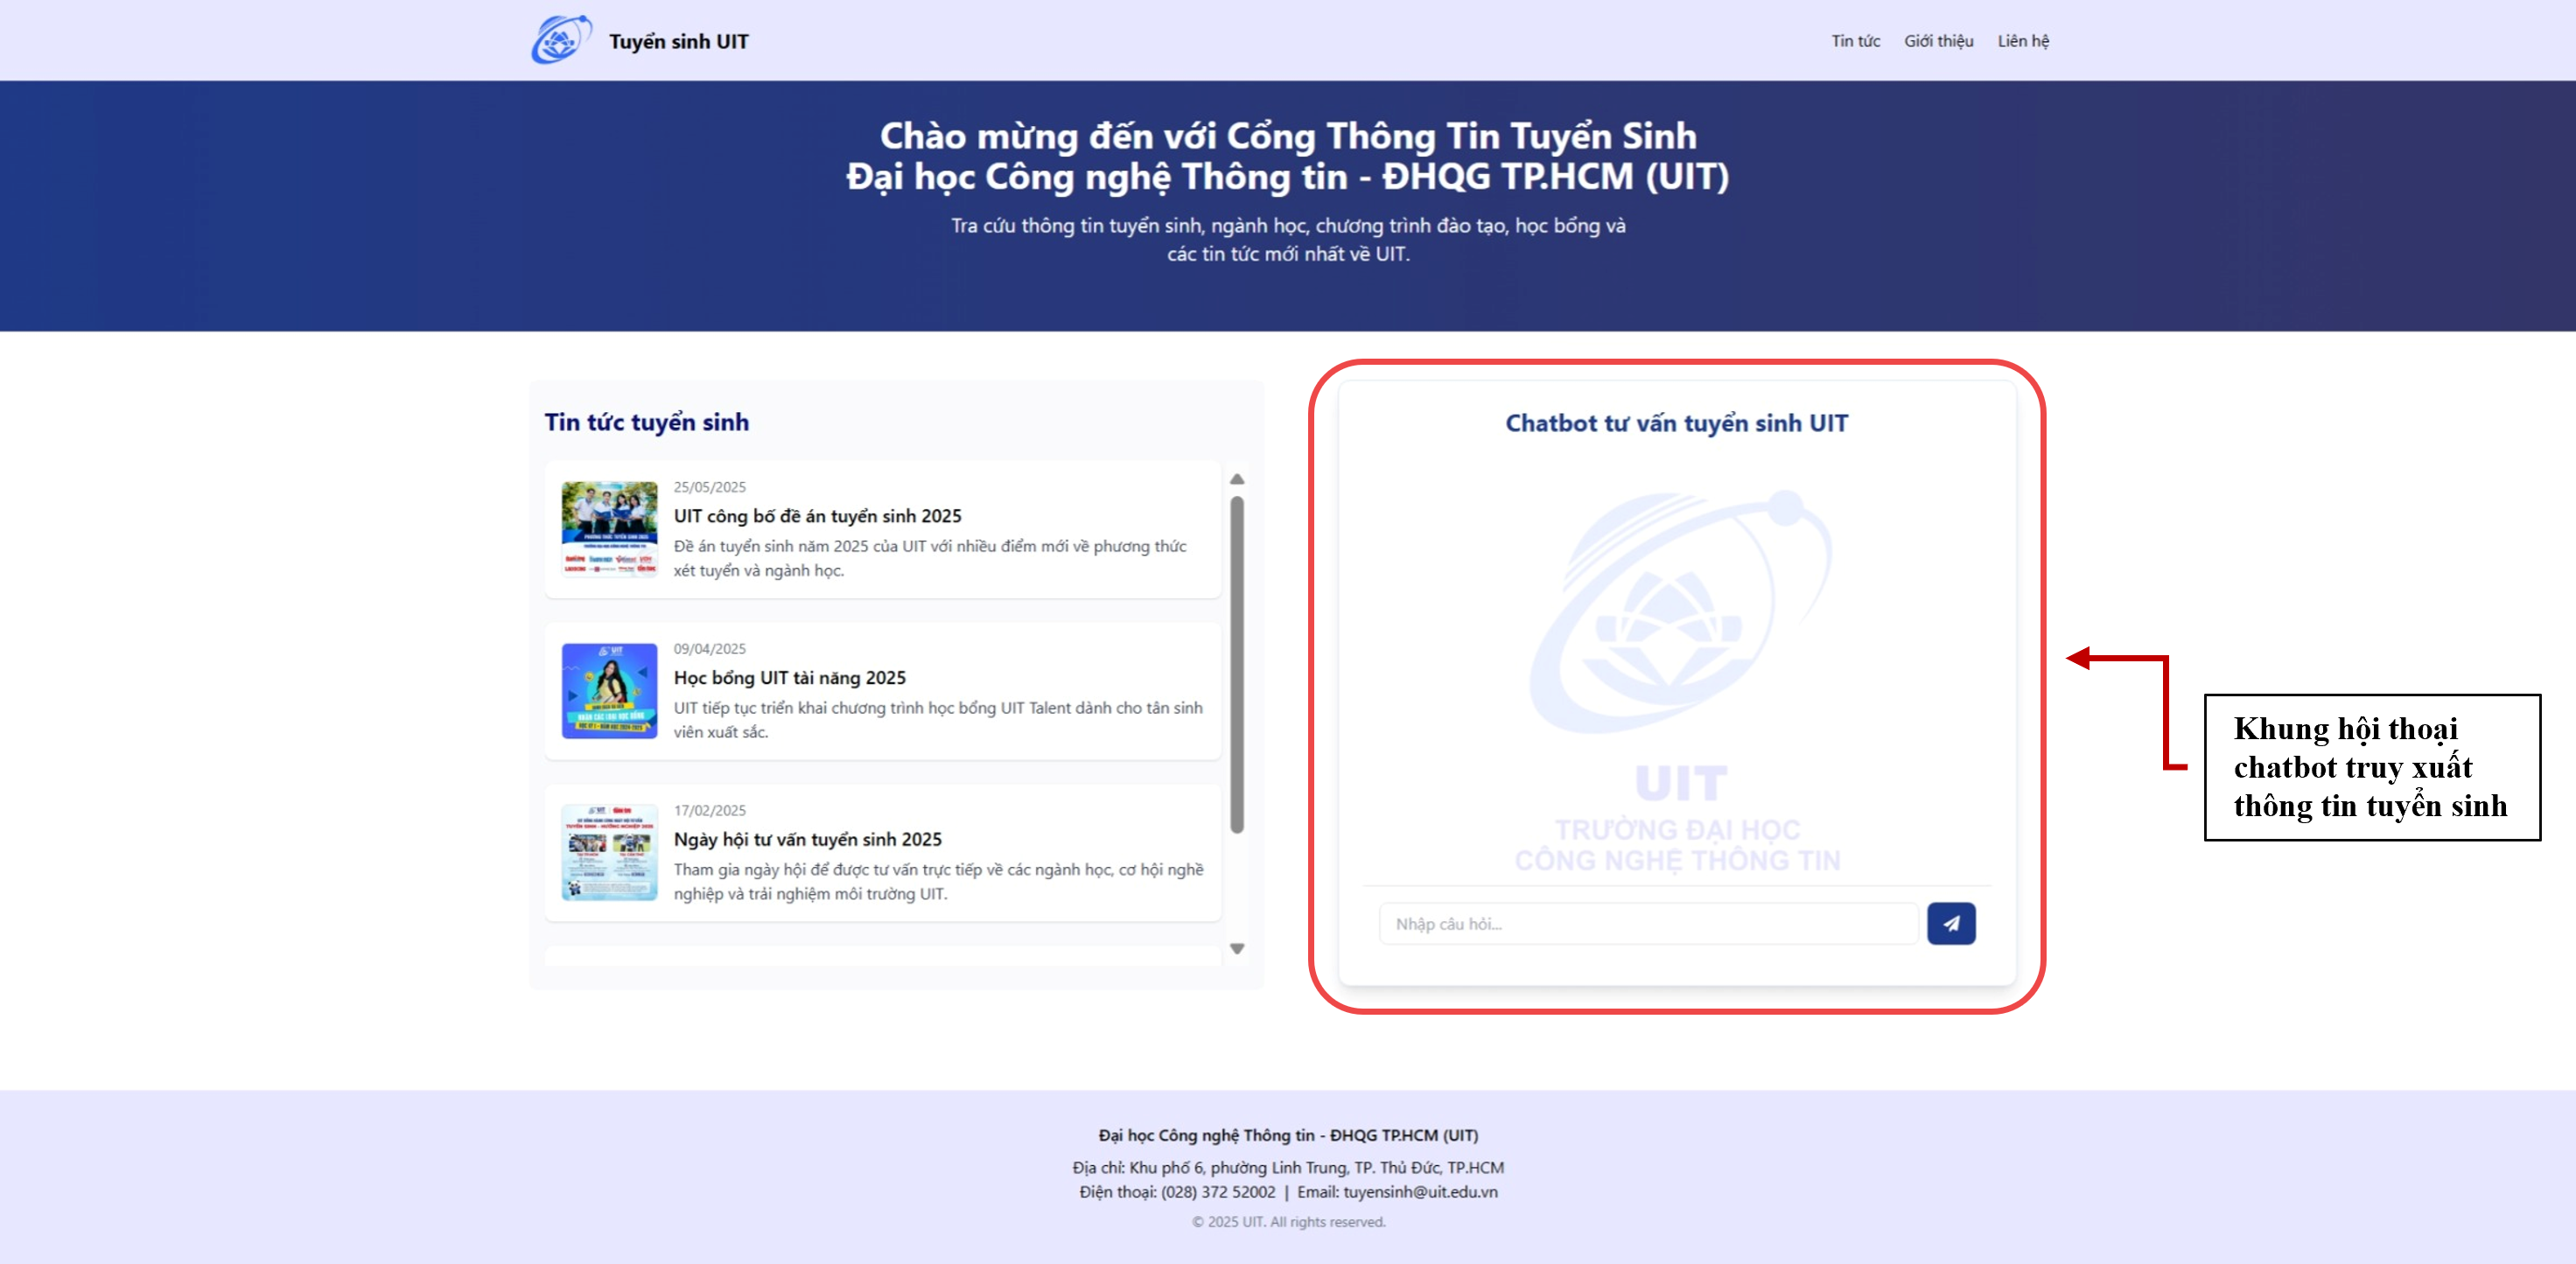
\includegraphics[width=\linewidth]{assets/app_demo.png}
    \end{center}
\end{figure}

\subsection{Công nghệ sử dụng}

Hệ thống được xây dựng với kiến trúc client-server, sử dụng các công nghệ hiện đại và phù hợp với các bài toán xử lý ngôn ngữ tự nhiên trong môi trường web. Cụ thể:

\begin{itemize}
    \item \textbf{Ngôn ngữ và nền tảng:} Toàn bộ hệ thống phía máy chủ được phát triển bằng Python, sử dụng \textbf{Django REST Framework} để xây dựng các dịch vụ API. Phía giao diện người dùng sử dụng \textbf{React với TypeScript}, triển khai theo hướng component hóa, hỗ trợ thiết kế phản hồi (responsive) và tương tác thời gian thực.

    \item \textbf{Cơ sở dữ liệu:} Hệ thống sử dụng \textbf{PostgreSQL (Neon)} cho dữ liệu quan hệ và \textbf{Qdrant} làm cơ sở dữ liệu vector chuyên biệt cho truy xuất ngữ nghĩa. Qdrant hỗ trợ tìm kiếm nhanh dựa trên khoảng cách giữa các embedding vector.

    \item \textbf{Xử lý ngôn ngữ và truy xuất:} Dữ liệu được biểu diễn bằng mô hình embedding tiếng Việt \texttt{AITeamVN/Vietnamese\_Embedding}. Việc phân đoạn tài liệu và quản lý ngữ cảnh được thực hiện thông qua thư viện \textbf{LangChain}.

    \item \textbf{Sinh phản hồi:} Hệ thống tích hợp \textbf{Google Cloud Generative AI} để sinh câu trả lời hội thoại dựa trên ngữ cảnh đã truy xuất.

    \item \textbf{Kết nối và giao tiếp:} Frontend sử dụng thư viện \textbf{Axios} để tương tác với các dịch vụ phía backend thông qua các endpoint RESTful.
\end{itemize}

\section{Thu thập và xử lý dữ liệu}

\subsection{Web Crawling}

Quá trình thu thập dữ liệu được thực hiện thông qua module \texttt{crawler.py}, cho phép tự động thu thập toàn bộ nội dung liên quan trên trang tuyển sinh của UIT chỉ với một tham số đầu vào là đường dẫn gốc:

\begin{center}
    \texttt{base\_url = `https://tuyensinh.uit.edu.vn/'}
\end{center}

Thuật toán thực hiện việc truy cập vào địa chỉ chính, trích xuất các liên kết có trong trang, và lần lượt tiếp tục thu thập theo hướng duyệt theo chiều rộng trong cùng miền. Tại mỗi liên kết, nội dung chính được xác định thông qua các bộ chọn cấu trúc HTML, sau đó được chuyển đổi sang định dạng Markdown phục vụ cho quá trình xử lý tiếp theo.

Quy trình crawling bao gồm:
\begin{itemize}
    \item Truy xuất nội dung HTML của từng trang.
    \item Trích xuất vùng nội dung chính, loại bỏ các thành phần không liên quan như điều hướng và chân trang.
    \item Chuyển đổi nội dung sang định dạng Markdown để lưu trữ.
    \item Tiếp tục thu thập các liên kết mới được tìm thấy trong trang và lặp lại quy trình.
\end{itemize}

Việc tự động hóa quy trình này giúp đảm bảo toàn bộ thông tin trên website tuyển sinh được thu thập một cách đầy đủ và dễ dàng mở rộng cho các website khác trong tương lai chỉ bằng cách thay đổi giá trị \texttt{base\_url}.


\subsection{Tiền xử lý dữ liệu}

Sau quá trình thu thập, dữ liệu văn bản ở định dạng Markdown được xử lý trước khi đưa vào mô hình embedding. Quá trình tiền xử lý bao gồm hai giai đoạn chính: làm sạch nội dung và phân chia tài liệu thành các đoạn nhỏ (chunk) phù hợp cho truy xuất ngữ nghĩa.

\subsubsection{Làm sạch Markdown}

Module \texttt{clean\_markdown.py} thực hiện các thao tác làm sạch định dạng Markdown nhằm chuẩn hoá nội dung và cấu trúc của tài liệu. Các bước xử lý bao gồm:

\begin{itemize}
    \item Loại bỏ các ký tự không mong muốn (whitespace thừa, ký hiệu ẩn, HTML tags).
    \item Chuẩn hoá hệ thống tiêu đề theo cấp độ (heading hierarchy) bằng cách ánh xạ các mục La Mã, mục đánh số sang cú pháp Markdown chuẩn.
\end{itemize}

\subsubsection{Phân đoạn tài liệu (Document Chunking)}

Sau khi nội dung được làm sạch, hệ thống thực hiện phân chia tài liệu thành các đoạn nhỏ bằng module \texttt{chunking.py}. Thuật toán sử dụng kỹ thuật Semantic Chunking từ thư viện LangChain để xác định ranh giới ngữ nghĩa giữa các đoạn. Cấu trúc tổng thể như sau:

\begin{itemize}
    \item Tài liệu đầu vào được phân tích theo các tiêu đề con (heading levels) để tạo thành các phần nội dung chính.
    \item Mỗi phần tiếp tục được chia nhỏ theo ngữ nghĩa sử dụng công cụ \texttt{Semantic\allowbreak{}Chunker} kết hợp với mô hình embedding tiếng Việt \texttt{AITeamVN/\allowbreak{}Vietnamese\_\allowbreak{}Embedding}.
    \item Mỗi đoạn nhỏ (chunk) được gắn kèm thông tin tiêu đề, nguồn, từ khóa và nhãn phân loại chủ đề.
\end{itemize}

\subsubsection{Phân loại theo chủ đề}

Hệ thống tích hợp cơ chế gán nhãn chủ đề tự động cho mỗi đoạn dựa trên tập từ khóa xác định trước. Một số chủ đề chính bao gồm:

\begin{itemize}
    \item \textbf{Ngành học:} như An toàn thông tin, Khoa học dữ liệu, Trí tuệ nhân tạo, etc.
    \item \textbf{Tuyển sinh:} điểm chuẩn, phương thức xét tuyển, chỉ tiêu, điều kiện.
    \item \textbf{Học bổng:} các loại học bổng, tiêu chí, quy trình xét duyệt.
    \item \textbf{Thông tin trường:} giới thiệu giảng viên, cơ sở vật chất, hoạt động sinh viên.
\end{itemize}

Việc gán nhãn được thực hiện bằng cách so khớp từ khóa theo cả dạng có dấu và không dấu, kết hợp với ưu tiên các từ xuất hiện sớm trong văn bản để tăng tính chính xác trong phân loại.

\section{Hệ thống Tìm kiếm Kết hợp (Hybrid Search)}

Hệ thống truy xuất thông tin trong dự án được thiết kế theo hướng kết hợp (hybrid), tích hợp đồng thời hai phương pháp: truy xuất ngữ nghĩa dựa trên vector embedding và truy xuất truyền thống dựa trên mô hình BM25. Cách tiếp cận này cho phép tận dụng được điểm mạnh của từng phương pháp: khả năng hiểu ngữ cảnh sâu của mô hình học sâu và tính chính xác của từ khóa trong các truy vấn cụ thể.

\subsection{Truy xuất ngữ nghĩa (Semantic Search)}

Các đoạn văn bản sau khi được xử lý sẽ được ánh xạ thành các vector ngữ nghĩa sử dụng mô hình \texttt{AITeamVN/Vietnamese\_Embedding}. Việc ánh xạ được thực hiện thông qua lớp \texttt{DocEmbedder}, trong đó mỗi đoạn được tổ hợp từ tiêu đề, tiêu đề mục và nội dung thân nhằm tăng độ bao phủ ngữ cảnh.

Các vector sau khi sinh được lưu trữ trong cơ sở dữ liệu vector Qdrant, sử dụng thuật toán lập chỉ mục \texttt{HNSW (Hierarchical Navigable Small World Graph)}. HNSW là một cấu trúc đồ thị đa tầng cho phép tìm kiếm gần đúng với độ chính xác cao, bằng cách duyệt từ tầng cao nhất (ít điểm, khoảng cách xa) xuống tầng thấp hơn (nhiều điểm, khoảng cách gần hơn). Việc tìm kiếm được thực hiện bằng phép đo \texttt{cosine similarity} giữa vector truy vấn và các vector tài liệu.

Mỗi vector được lưu kèm một \textit{payload} chứa metadata như tiêu đề, ngành học, năm, và nguồn gốc nội dung. Ngoài chỉ mục vector, Qdrant còn hỗ trợ các chỉ mục phụ (payload index) để lọc theo điều kiện cụ thể, ví dụ: chỉ lấy các đoạn liên quan đến ``tuyển sinh năm 2024''.

\subsection{Truy xuất theo mô hình BM25}

Song song với truy xuất ngữ nghĩa, hệ thống cũng tích hợp mô hình \texttt{BM25} - một cải tiến của TF-IDF

Quá trình xử lý văn bản cho BM25 bao gồm:

\begin{itemize}
    \item Chuẩn hóa văn bản: loại bỏ ký tự đặc biệt và stopwords, chuyển về chữ thường.
    \item Token hóa tiếng Việt bằng thư viện \texttt{pyvi}.
    \item Sinh n-gram ngữ cảnh để tăng độ bao phủ truy vấn (với kích thước cửa sổ ngữ cảnh là 2).
\end{itemize}

\subsection{Cơ chế kết hợp điểm số}

Hai điểm số truy xuất từ mô hình ngữ nghĩa và mô hình BM25 được kết hợp theo công thức sau:
\[
    \text{final\_score} = \alpha \cdot \text{semantic\_score} + (1 - \alpha) \cdot \text{bm25\_score\_normalized}
\]

Người dùng hoặc hệ thống có thể điều chỉnh tham số \(\alpha\) nhằm ưu tiên một phương pháp hơn trong các ngữ cảnh truy vấn khác nhau. Ví dụ, nếu \(\alpha = 1\) thì hệ thống sẽ thực hiện truy xuất hoàn toàn theo hướng ngữ nghĩa; ngược lại, nếu \(\alpha = 0\), chỉ có điểm BM25 được sử dụng.

Việc kết hợp hai hướng truy xuất này giúp tăng độ linh hoạt và độ chính xác của hệ thống.

\subsection{Các tính năng khác}

\subsubsection{Lọc theo ngưỡng độ tin cậy (Confidence Thresholding)}

Để nâng cao chất lượng kết quả truy xuất, hệ thống áp dụng cơ chế lọc theo ngưỡng độ tin cậy kép. Cụ thể, mỗi kết quả truy xuất chỉ được giữ lại nếu đồng thời thỏa mãn hai điều kiện:

\begin{itemize}
    \item Điểm truy xuất ngữ nghĩa (semantic score) phải lớn hơn hoặc bằng một ngưỡng xác định.
    \item Điểm BM25 cũng phải lớn hơn hoặc bằng một ngưỡng tối thiểu.
\end{itemize}

Cơ chế này giúp loại bỏ các đoạn văn bản có điểm ngữ nghĩa cao nhưng không chứa từ khóa rõ ràng liên quan, hoặc ngược lại — các đoạn chứa từ khóa nhưng không phù hợp ngữ cảnh truy vấn. Việc kết hợp cả hai tiêu chí giúp tăng độ chính xác và phù hợp của kết quả đầu ra, đặc biệt quan trọng trong các truy vấn tuyển sinh có tính đặc thù và yêu cầu chính xác cao.

\subsubsection{Phân tích từ khóa (Keyword Analysis)}

Ngoài truy xuất, hệ thống còn hỗ trợ chức năng phân tích và trích xuất các từ khóa quan trọng nhất trong mỗi đoạn văn bản (chunk). Dựa trên mô hình BM25, hệ thống tính toán mức độ quan trọng của từng từ khóa trong mỗi đoạn và liệt kê các từ có trọng số cao nhất. Việc hiển thị từ khóa có trọng số cao nhất theo từng đoạn (chunk) cũng có thể được sử dụng trong giai đoạn đánh giá hệ thống hoặc tinh chỉnh ngưỡng điểm để cải thiện hiệu quả truy xuất.

\section{Kết quả và đánh giá}

\subsection{Ví dụ truy vấn và kết quả sinh phản hồi}

Truy vấn người dùng: \textit{``Giới thiệu về ngành học Trí tuệ nhân tạo''}

\textbf{Các đoạn văn bản được truy xuất (top-5):}
\begin{itemize}
    \item \textbf{Tài liệu 1} (Score: 0.6405): ``\textit{Với sự phát triển như vũ bão của Cách mạng công nghệ 4.0, Trí tuệ nhân tạo (AI) trở thành ngành 'hot'...}''
    \item \textbf{Tài liệu 2} (Score: 0.6162): ``\textit{Nguồn: https://\allowbreak{}tuyensinh.uit.edu.vn/\allowbreak{}tong-quan-nganh-tri-tue-nhan-tao...}''
    \item \textbf{Tài liệu 3} (Score: 0.6038): ``\textit{Bộ môn có nhiệm vụ nghiên cứu khoa học và giảng dạy các môn học theo định hướng Trí tuệ nhân tạo...}''
    \item \textbf{Tài liệu 4} (Score: 0.5921): ``\textit{Chương trình đào tạo ngành Trí tuệ nhân tạo hướng đến mục tiêu đào tạo nguồn nhân lực chất lượng cao...}''
    \item \textbf{Tài liệu 5} (Score: 0.5909): ``\textit{Sau khi tốt nghiệp, sinh viên có thể làm việc: Chuyên gia lập trình Trí tuệ nhân tạo...}''
\end{itemize}

\textbf{Câu trả lời:}

\begin{quote}
    \small
    Ngành Trí tuệ Nhân tạo (AI) là một trong những ngành trọng điểm hiện nay, đóng vai trò then chốt trong Cách mạng công nghiệp 4.0. Trường Đại học Công nghệ Thông tin (UIT) chú trọng đào tạo đội ngũ nhân lực chất lượng cao trong lĩnh vực này.

    Thông tin chung: Tên ngành: Trí tuệ nhân tạo (Artificial Intelligence); Mã ngành: 7480107; Hệ đào tạo: chính quy; Thời gian: 3.5 năm.

    Mục tiêu đào tạo: Cung cấp nền tảng vững chắc về khoa học máy tính và chuyên sâu về AI; hình thành năng lực thiết kế, phát triển hệ thống thông minh; có thể tiếp tục học lên cao.

    Cơ hội nghề nghiệp: Làm việc trong lĩnh vực phát triển phần mềm AI, phân tích dữ liệu, nghiên cứu tại các trung tâm R\&D hoặc tiếp tục học cao học chuyên ngành AI.

    Lĩnh vực đào tạo chuyên sâu: Máy học, biểu diễn tri thức và suy luận, dữ liệu lớn, thuật toán tiến hóa, v.v.
\end{quote}

\textbf{Nhận xét:} Hệ thống đã truy xuất đúng các đoạn có liên quan ngữ nghĩa cao, kết hợp nội dung tốt để tạo phản hồi đầy đủ, đúng trọng tâm.

\subsection{Nhận xét và định hướng phát triển}

Mặc dù hệ thống đã hoạt động ổn định và sinh phản hồi tương đối chính xác cho các câu hỏi trong miền chủ đề tuyển sinh, vẫn tồn tại một số hạn chế cần khắc phục:

\begin{itemize}
    \item Hệ thống hiện tại vẫn truy xuất và đưa vào mô hình sinh phản hồi ngay cả khi truy vấn không liên quan đến chủ đề tuyển sinh. Việc đánh giá mức độ liên quan chủ yếu do mô hình ngôn ngữ lớn (LLM) đảm nhiệm, dẫn đến tình trạng lãng phí tài nguyên truy xuất và có thể tạo ra phản hồi sai nếu ngữ cảnh không phù hợp. Định hướng sắp tới là tích hợp thêm một mô hình học máy nhẹ để phân loại truy vấn ngay từ đầu, chỉ thực hiện truy xuất khi truy vấn thực sự liên quan, từ đó tiết kiệm tài nguyên và nâng cao độ chính xác.

    \item Mở rộng dữ liệu: Tìm thêm các trang base\_url để có thể có thêm các thông tin liên quan đến tuyển sinh hoặc các thông tin về trường...

    \item Nâng cao chiến lược lọc nội dung: Sử dụng các công cụ như \texttt{KeyBERT} để trích xuất từ khóa chủ đề và áp dụng cơ chế lọc cứng (hard filtering) trước khi truy xuất, giúp loại bỏ các đoạn không liên quan.

    \item Tối ưu hiệu năng: Giảm thời gian truy xuất và sinh phản hồi bằng cách tinh chỉnh vector index và giảm số lượng đoạn văn cần đưa vào LLM.
\end{itemize}

Hướng đi này sẽ giúp hệ thống trở nên chính xác hơn, phù hợp hơn với mục tiêu hỗ trợ tuyển sinh thực tế và nâng cao trải nghiệm người dùng trong môi trường web tương tác.
